\section{Implementierung eines Modells}
\label{sec:ModellImplementierung}
Bisher wurden die Grundlagen von neuronalen Netzen behandelt und der Datensatz ist vorbereitet.
Daher kann nun ein Modell definiert und implementiert werden, das die Vorhersage mobiler Radarkontrollen bewerkstelligt.
In diesem Abschnitt wird das Modell außerdem trainiert und evaluiert.
Zudem werden einige weitere praktische Aspekte erläutert und das Modell optimiert.

\subsection{Definition des Modells}
\label{sec:ModellDefinition}
Ziel dieses Unterabschnitts ist es herauszuarbeiten, wie mehrere ConvLSTM-Layer zusammen mit anderen Layertypen für räumlich-zeitliche Vorhersagen verwendet werden können.
Außerdem wird eine Verlustfunktion definiert, die für den vorliegenden Anwendungsfall geeignet ist.

ConvLSTM-Layer können unterschiedlich verwendet werden, um bestimmte Anwendungsfälle abzudecken.
Die wichtigste Unterscheidung ist, ob die Ausgabe des Modells eine Sequenz oder ein einzelner 2D-Tensor sein soll.
Der erste Fall wird beispielsweise für die Weiterführung einer Bildsequenz verwendet, wie in \cite{VideoPredKeras} demonstriert.
Eine solche Architektur könnte im Kontext der vorliegenden Arbeit beispielsweise verwendet werden, um die Gefahr für mobile Radarkontrollen mehrere Tage vorauszusagen.
Dies ist jedoch hier nicht notwendig.
Eine alternative Architektur wird in \cite{CrimeConvLSTM} vorgestellt.
Diese ist dazu in der Lage, anhand einer Sequenz von 16 oder 32 2D-Eingangstensoren den folgenden 2D-Tensor vorherzusagen.
Die Architektur wurde im Kontext der Verbrechensvorhersage entwickelt.
Da es sich dabei ebenfalls um sporadisch auftretende Ereignisse handelt, ist die Architektur mit hoher Wahrscheinlichkeit auch für den vorliegenden Anwendungsfall geeignet.
Die Architektur ist in \autoref{fig:ArchCrimeConvLSTM} dargestellt.

\begin{figure}[ht!]
    \centering
    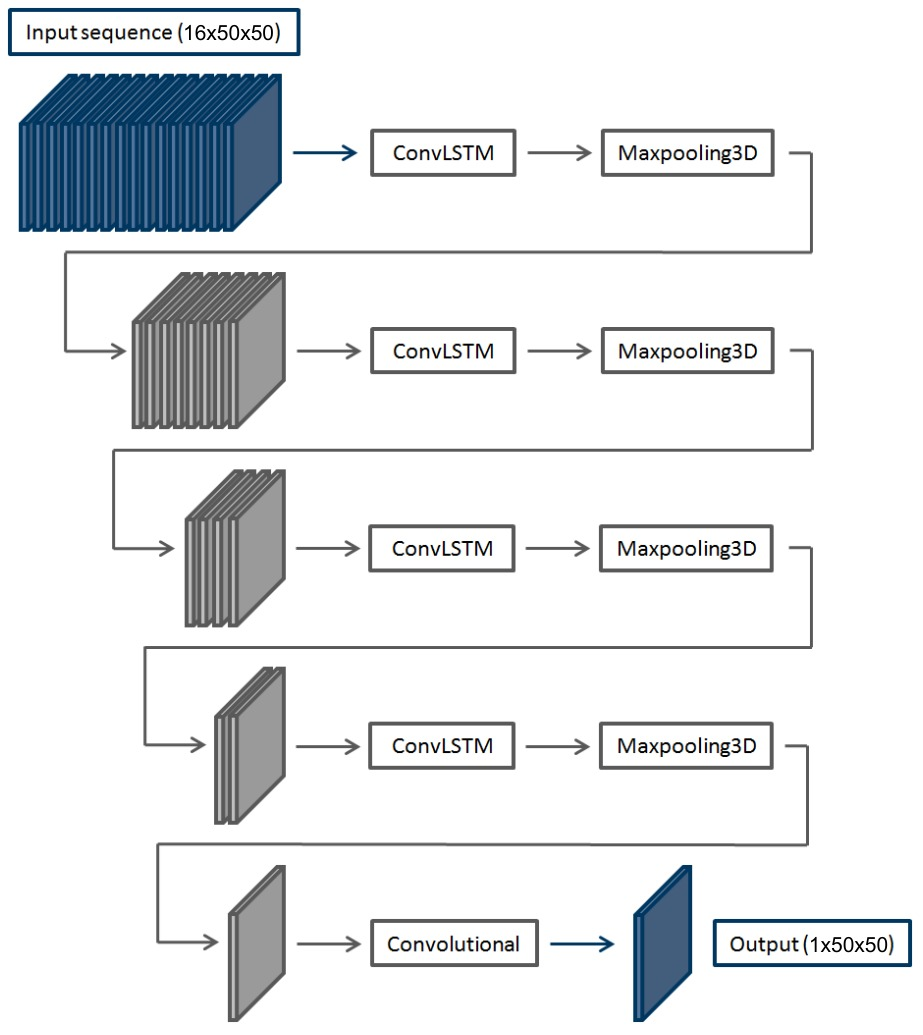
\includegraphics[width=1.0\textwidth,height=16cm,keepaspectratio=true]{content/images/ArchCrimeConvLSTM.jpeg}
    \caption{Architektur eines Modells aus mehreren ConvLSTM- und MaxPooling-Layern nach \cite[Figure 2.1]{CrimeConvLSTM} mit angepassten Dimensionen}
    \label{fig:ArchCrimeConvLSTM}
\end{figure}

Anhand der Abbildung kann der Datenfluss verfolgt werden.
Wie ganz oben zu erkennen ist, hat die Eingabesequenz eine Größe von 16x50x50.
Die Eingabe ist also eine Sequenz von 16 Frames, die jeweils 50x50 Pixel groß sind.
Es ist anzumerken, dass die Eingabesequenz in \cite{CrimeConvLSTM} die Dimensionen 50x50x16 hat.
Die erste und letzte Dimension ist für die vorliegende Arbeit getauscht, da die Verarbeitung so intuitiver ist.
Das Resultat ist jedoch dasselbe.
Die Eingabe durchläuft nun mehrmals je einen ConvLSTM- und einen MaxPooling3D-Layer.
Die ConvLSTM-Layer haben nach \cite{CrimeConvLSTM} eine Kernelgröße von 3x3 Pixel.
Außerdem werden Höhe und Breite der Frames durch Padding beibehalten.
Auch die Anzahl an Frames bleiben durch die ConvLSTM-Layer erhalten.
Um von den 16 Frames auf ein Frame als Ausgang zu kommen, befindet sich hinter jedem ConvLSTM-Layer ein MaxPooling3D-Layer.
Dieser Layer berechnet je das Maximum zweier Pixel, die in zwei benachbarten Frames an derselben Position liegen.
Dies entspricht einer Poolgröße von $(2, 1, 1)$.
Außerdem wird eine Schrittweite von $(2, 1, 1)$ verwendet.
Das Resultat ist (vereinfacht auf 3x3 Pixel) in \autoref{fig:MaxPooling3D} dargestellt.

\begin{figure}[ht!]
    \centering
    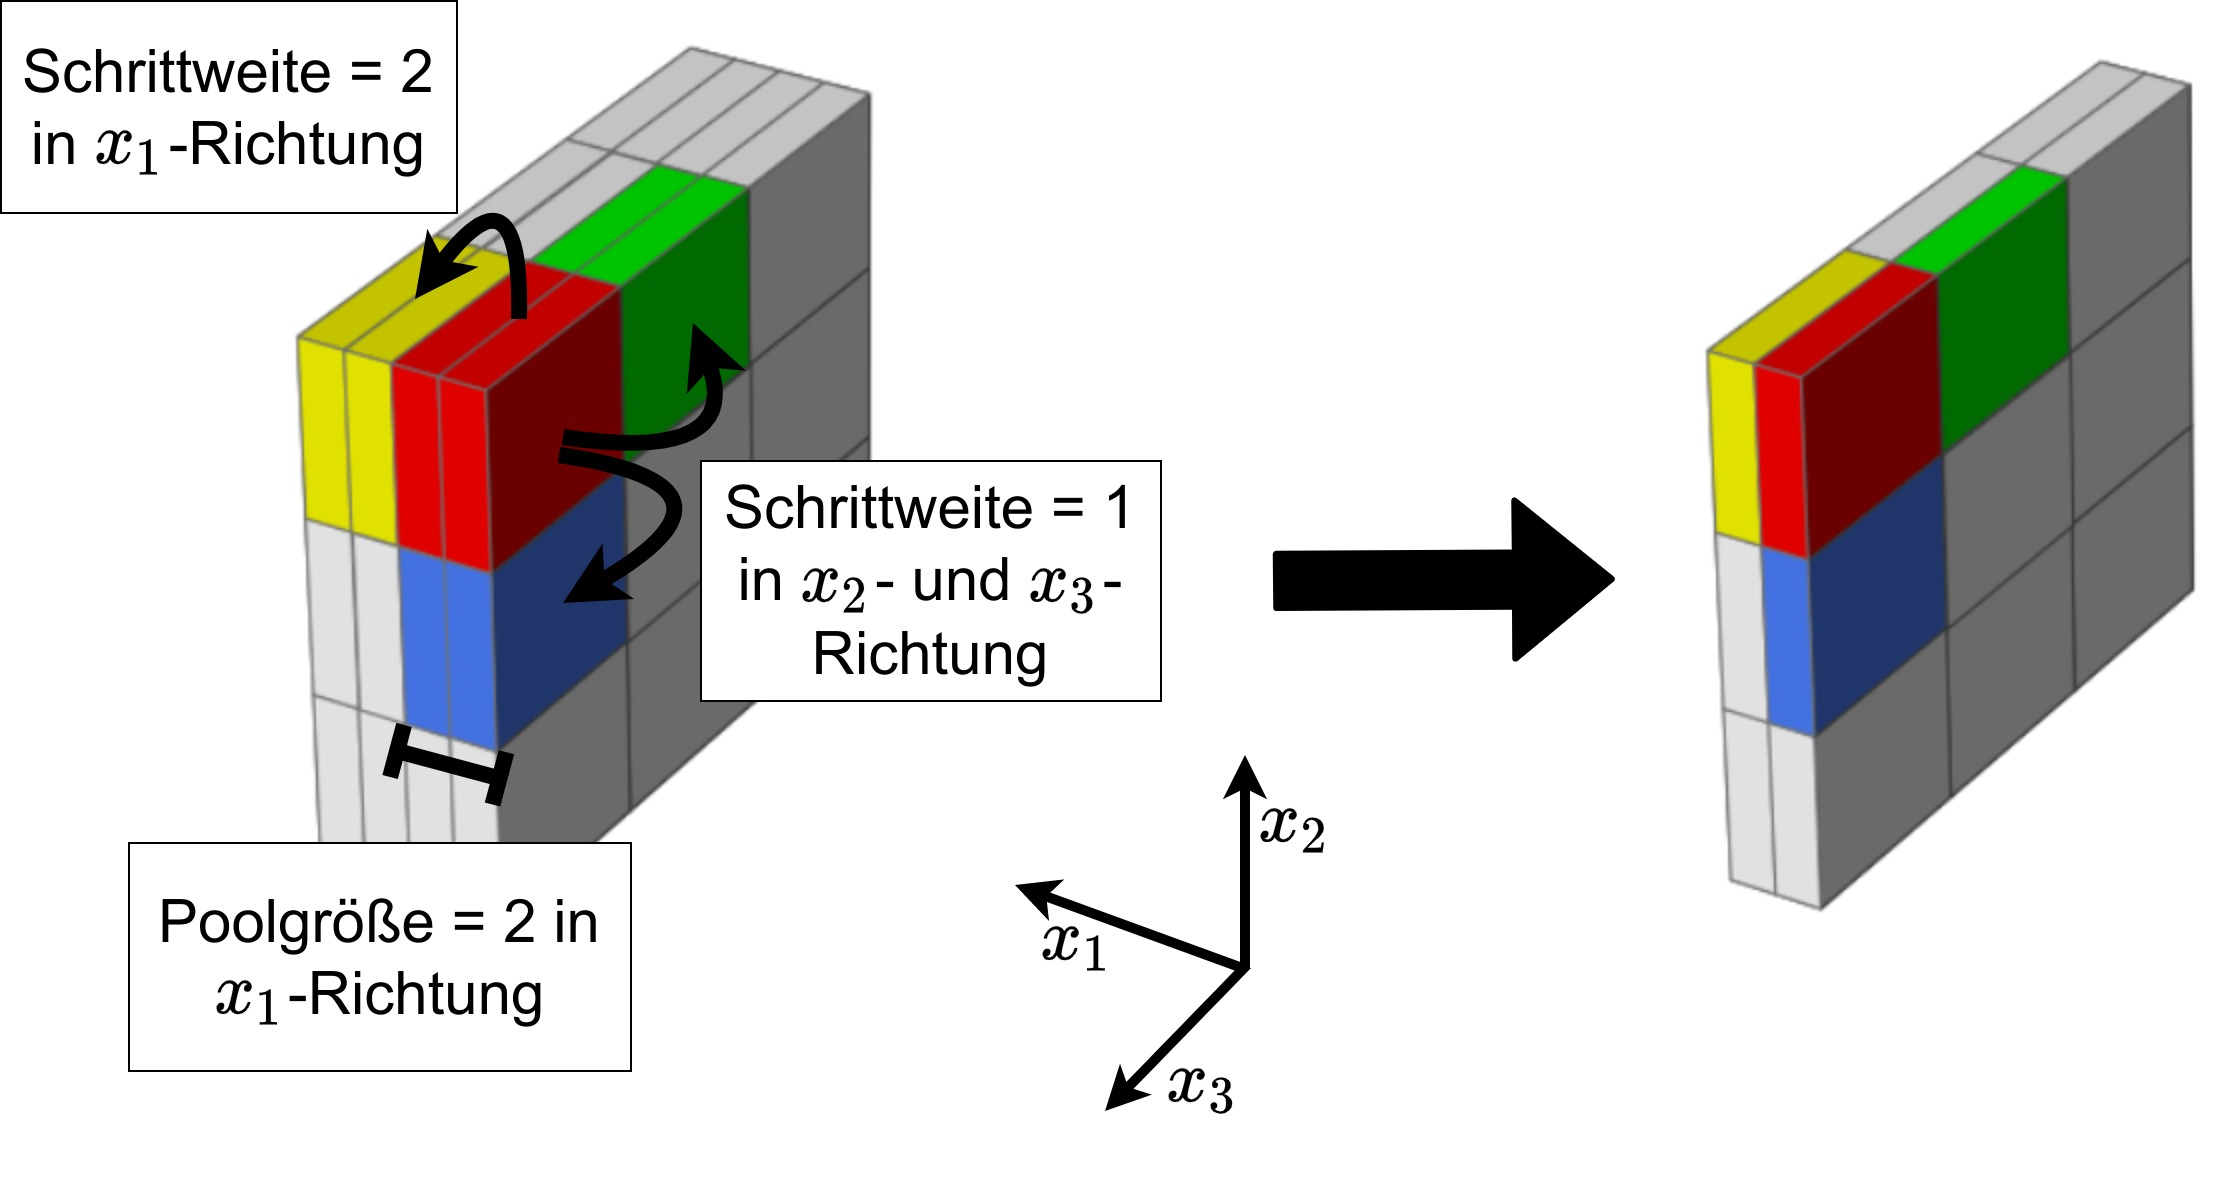
\includegraphics[width=0.8\textwidth,height=8cm,keepaspectratio=true]{content/images/MaxPooling3D.jpeg}
    \caption{Visualisierung der MaxPooling3D-Operation mit einer Poolgröße von $(2, 1, 1)$ und einer Schrittweite von $(2, 1, 1)$ anhand von vier Eingangsframes zu je 3x3 Pixeln}
    \label{fig:MaxPooling3D}
\end{figure}

Mit der MaxPooling3D-Operation werden damit die signifikantesten Merkmale von je zwei benachbarten Frames vereint.
Dadurch wird die Anzahl der Frames in der Sequenz nach jeder ConvLSTM-MaxPooling3D-Kombination halbiert.
Somit ist nach vier dieser Kombinationen nur noch ein Frame übrig.
Am Ende liegt nach \cite{CrimeConvLSTM} noch ein 3D-Faltungslayer mit einer Kernelgröße von $(1, 3, 3)$.
Dort ist die dreidimensionale Version eines Faltungslayers nötig, da die erste und letzte Dimension wie oben angemerkt vertauscht ist.
Da ein 3D-Faltungslayer mit einer Kernelgröße von $(3, 3, 1)$ (wie er hier verwendet werden müsste) exakt einem 2D-Faltungslayer mit einer Kernelgröße von $(3, 3)$ entspricht, wird hier letzterer verwendet.

Um das Modell trainieren zu können muss noch eine Verlustfunktion ausgewählt werden.
Dafür könnte eine gewöhnliche Verlustfunktion für die Klassifizierung wie die binäre Kreuzentropie (engl. \emph{binary cross entropy}) verwendet werden.
Das liegt daran, dass der vorliegende Anwendungsfall als Binärklassifizierung angesehen werden kann: entweder es befindet sich eine Radarkontrolle in einer Rasterzelle oder nicht.
Bei einem ausgeglichenen Datensatz könnte eine solche Verlustfunktion direkt verwendet werden.
Für den vorliegenden Anwendungsfall ist jedoch die Besonderheit zu beachten, dass es in den Daten deutlich mehr Rasterzellen ohne eine einzige Radarkontrolle gibt als Rasterzellen, in denen es mindestens eine gibt.
Mit einer normalen Verlustfunktion werden falsch-negative Ergebnisse genauso hart bestraft wie falsch-positive.
Andersherum werden richtig-positive Ergebnisse genauso begünstigt wie richtig-negative.
Hier ergibt sich jedoch ein Problem.
Ein bei der Trainierung sehr schnell zu findendes Minimum der Verlustfunktion liegt genau dort, wo die Vorhersage des gesamten Rasters "`negativ"' ist.
Somit kann beispielsweise bei einer Positivenrate von 5\,\% im Datensatz eine Genauigkeit (engl. \emph{accuracy}) von 95\,\% erzielt werden, wenn alle Rasterzellen als "`negativ"' vorhergesagt werden.
Allerdings entsteht damit keinerlei Erkenntnisgewinn.
Damit der Optimierungsalgorithmus nicht nach kurzer Zeit in dieses schnell zu erreichende Minimum fällt, kann nach \cite{CrimeConvLSTM} eine gewichtete Verlustfunktion verwendet werden.
Eine gewichtete Verlustfunktion weist den einzelnen Klassen Gewichtungen zu, die mit den Kreuzentropiewerten der jeweiligen Klasse multipliziert werden.
Ist die Gewichtung größer als $1$, wird der Wert der Kreuzentropie verstärkt bzw. mehr gewichtet und umgekehrt.
Die in der vorliegenden Arbeit verwendete Verlustfunktion ist in \autoref{lst:WeightedCrossEntropy} dargestellt.

\begin{code}
\begin{minted}[
    linenos,
    numbersep=10pt,
    gobble=0,
    frame=lines,
    framesep=2mm]{python}
def weighted_binary_crossentropy(weights: dict):
    def loss_fn(y_true, y_pred):
        tf_y_true = tf.cast(y_true, dtype=y_pred.dtype)
        tf_y_pred = tf.cast(y_pred, dtype=y_pred.dtype)

        weights_v = tf.where(tf.equal(tf_y_true, 1), weights[1], weights[0])
        crossentropy = K.binary_crossentropy(tf_y_true, tf_y_pred)
        weighted_crossentropy = tf.multiply(crossentropy, weights_v)

        loss = K.mean(weighted_crossentropy)
        return loss

    return loss_fn
\end{minted}
\captionof{listing}{Implementierung einer gewichteten Kreuzentropie als Verlustfunktion für spärliche Daten}
\label{lst:WeightedCrossEntropy}
\end{code}

In Zeile 6 wird die Matrix \emph{weights\_v} berechnet, die die Gewichtungen jeweils an den Stellen enthalten, an denen die jeweilige Klasse in den wahren Daten vorkommen.
In Zeile 7 wird die gewöhnliche binäre Kreuzentropie berechnet.
In Zeile 8 werden dann die Gewichtungen durch elementweise Multiplikation zu den Vorkommnissen der jeweiligen Klasse multipliziert.
Die Matrix \emph{weighted\_crossentropy} enthält nun die gewichtete Kreuzentropie für jeden Datenpunkt, also jede Rasterzelle.
Der Verlustwert berechnet sich dann in Zeile 10 aus dem Durchschnitt aller dieser Werte.

Als nächstes stellt sich noch die Frage, welche Gewichtungen verwendet werden sollten.
Nach \cite{KerasImbalancedData} bietet es sich an, die Gewichtungen anhand der Anzeile der verschiedenen Klassen am gesamten Datensatz zu berechnen.
Somit sind die Gewichtungen abhängig von der konkreten Beschaffenheit des Datensatzes.
Konkret wird in \cite{KerasImbalancedData} die Implementierung vorgeschlagen, die in \autoref{lst:ClassWeights} zu sehen ist.

\begin{code}
\begin{minted}[
    linenos,
    numbersep=10pt,
    gobble=0,
    frame=lines,
    framesep=2mm]{python}
def get_class_weights(dataset):
    neg, pos = np.bincount(dataset.flatten())
    total = neg + pos
    weight_for_0 = (1.0 / neg) * (total / 2.0)
    weight_for_1 = (1.0 / pos) * (total / 2.0)

    return weight_for_0, weight_for_1
\end{minted}
\captionof{listing}{Berechnung der Klassengewichtungen nach \cite{KerasImbalancedData}}
\label{lst:ClassWeights}
\end{code}

In Zeile 2 wird mit \emph{np.bincount()} die Anzahl an "`0"'- und "`1"'-Werten im gesamten Datensatz berechnet.
In Zeile 4 und 5 werden dann die Gewichtungen berechnet, sodass diese reziprok proportional zum Anteil der Klassen sind.
Nach die Skalierung um \emph{total/2} bewirkt dabei, dass der Absolutwert des Verlusts nicht zu groß bzw. zu klein wird, um ihn als Mensch noch einigermaßen interpretieren zu können.
In einem zufälligen Teil des Radarkontrollen-Datensatzes sind beispielsweise 5.09\,\% der Rasterzellen "`positiv"'.
Daraus ergeben sich die Gewichtungen $0,53$ für die Klasse "`0"' und $9,83$ für die Klasse "`1"'.

Mit der Netzarchitektur und der Verlustfunktion sind nun alle Bestandteile des Modells definiert.
Die Definition des Modells in TensorFlow ist in \appendixref{sec:ModellDefTF} zu sehen.
In den folgenden Abschnitten kann nun mit der Trainierung des Modells begonnen werden.

\subsection{Laden und vorbereiten des Datensatzes}
\label{sec:DatensatzLaden}
Um den Datensatz als Trainingsdaten für das neuronale Netz zu verwenden, muss er in ein numpy-Array geladen werden.
Zunächst ist das Ziel, die Frames des gesamten Datensatzes in ein numpy-Array mit der Form $(x,~50,~50)$ zu bringen, wobei $x$ der Anzahl an Frames entspricht.
Dafür kann der Code aus \autoref{lst:GdalOpen} verwendet werden, wobei über jedes Datum vom 17.07.2014 bis 25.10.2021 iteriert wird.
Somit ergibt sich ein Array der Form $(2652,~50,~50)$.
Die einzelnen Pixel enthalten bisher noch die summierte Standdauer der Radarkontrollen.
Mit dem Wissen um die gewichtete Verlustfunktion ist jedoch klar geworden, dass es sich bei der Problemstellung eigentlich um eine Binärklassifizierung handelt.
Daher muss nun ein Grenzwert ausgewählt werden, ab dem eine Rasterzelle als "`positiv"' gilt.
Auch hier muss zwischen der Verlässlichkeit der Meldungen und der Anzahl an positiven Datenpunkten abgewogen werden.
Da es jedoch wichtiger ist, alle künftigen Radarkontrollen vorherzusagen als alle Rasterzellen korrekt vorherzusagen, in denen es keine Radarkontrolle gibt, sollte der Grenzwert relativ niedrig gewählt werden.
Im Bezug auf die Verteilung der Standdauer in \autoref{fig:StanddauerVerteilung} scheint eine halbe Stunde ein guter Grenzwert zu sein.
Damit wird ein Großteil der Meldungen eingeschlossen, wobei die wenig verlässlichen Meldungen unter einer halben Stunde vernachlässigt werden.
Die Klassenzuordnung je nach Überschreitung des Grenzwertes kann mit numpy einfach implementiert werden als \emph{dataset = np.where(dataset > 0.5, 1, 0)}.

Als Nächstes muss der Datensatz in Sequenzen von je 17 Frames aufgeteilt werden, von denen die ersten 16 als Eingabesequenz dienen und das letzte als Zielframe.
Da die Vorhersage von beliebigen Wochentagen möglich sein soll und möglichst viele Trainingsdaten benötigt werden, sollten auch die Sequenzen ausgenutzt werden, die sich überschneiden.
Somit soll beispielsweise aus dem Array $[1,~2,~3,~4]$ bei einer Sequenzlänge von $2$ nicht nur das Array $[[1,~2], [3,~4]]$ entstehen, sondern das Array $[[1,~2],~[2,~3],~[3,~4]]$.
Wird der Datensatz auf diese Weise in Sequenzen unterteilt, entsteht ein Array der Form $(2636,~17,~50,~50)$.
Das Array enthält nun also 2636 Sequenzen aus je 17 Frames mit einer Größe von 50x50 Pixel.
Als Nächstes müssen die Sequenzen in zufällige Trainings- und Validierungsdaten unterteilt werden.
Dazu werden die Sequenzen zufällig gemischt und anschließend werden 90\,\% der Frames dem Trainingsdatensatz zugewiesen und 10\,\% den Validierungsdatensatz.
Die Sequenzen müssen im letzten Schritt noch je in die Ein- und Zielausgabe des \acrshortpl{nn} unterteilt werden.
Dies wird in \autoref{lst:CreateXYFrames} von der Funktion \emph{create\_xy\_frames()} implementiert.

\begin{minipage}{\textwidth}
\begin{code}
\begin{minted}[
    linenos,
    numbersep=10pt,
    gobble=0,
    frame=lines,
    framesep=2mm,
    escapeinside=!!]{python}
def create_xy_frames(data):
    x = data[:, 0:-2, :, :] !\label{x_frames}!
    y = data[:, -1, :, :] !\label{y_frames}!
    y = np.expand_dims(y, axis=1) !\label{y_frames_dim}!
    return x, y

x_train, y_train = create_xy_frames(train_dataset)
x_val, y_val = create_xy_frames(val_dataset)
\end{minted}
\captionof{listing}{Implementierung der Funktion \emph{create\_xy\_frames()} zum Unterteilen der Sequenzen in Eingabe und Zielausgabe}
\label{lst:CreateXYFrames}
\end{code}
\end{minipage}

In Zeile \ref{x_frames} wird zunächst die Eingabesequenz extrahiert.
Diese besteht aus dem ersten bis vorletzten Frame, somit hat der Eingabedatensatz \emph{x\_train} schließlich die Form $(2372,~16,~50,~50)$.
Die Zielausgabe hingegen wird in Zeile \ref{y_frames} erstellt und besteht nur aus dem letzten Frame jeder Sequenz.
Durch die Auswahl nur eines Elements einer Dimension geht diese Dimension jedoch komplett verloren.
Da das \acrshort{nn} die Dimension jedoch erwartet, muss sie in Zeile \ref{y_frames_dim} wieder hinzugefügt werden, sie hat dann die Länge $1$.
Damit hat die Zielausgabe \emph{y\_train} die Form $(2372,~1,~50,~50)$.
Nun sind die Trainingsdaten bereit und das Modell kann damit trainiert werden.

\subsection{Trainierung des Modells}
\label{sec:Trainierung}
Für die Trainierung werden zunächst noch zwei Callbacks definiert, um den Trainingsprozess zu verbessern.
Callbacks sind Funktionen, die nach jeder Epoche des Trainings aufgerufen werden.
Diese erhalten das Modell bei jedem Aufruf in seinem momentanen Zustand.
Daraufhin können Callbacks das Modell beispielsweise auf Testdaten anwenden, die Parameter des Trainings verändern oder das Training beenden.
Ein hilfreicher Callback ist \emph{EarlyStopping}.
Dieser überwacht die Performance des Modells mithilfe einer beliebigen Metrik und beendet das Training, wenn sich die Metrik nicht mehr signifikant verbessert \cite{KerasEarlyStopping}.
Somit kann überflüssige Trainingszeit gespart und Überanpassung vermieden werden.
Die Definition des Callbacks ist in \autoref{lst:ModelTraining} in Zeile 1 und 2 zu sehen.

\begin{code}
\begin{minted}[
    linenos,
    numbersep=10pt,
    gobble=0,
    frame=lines,
    framesep=2mm,
    escapeinside=!!]{python}
early_stopping = keras.callbacks.EarlyStopping(monitor="val_loss",
    patience=10, restore_best_weights=True)
reduce_lr = keras.callbacks.ReduceLROnPlateau(monitor="val_loss", patience=5)

epochs = 32
batch_size = 12
!\label{fit_start}!history = model.fit(
    x_train, y_train,
    batch_size=batch_size, epochs=epochs,
    validation_data=(x_val, y_val),
!\label{callbacks_passing}!    callbacks=[early_stopping, reduce_lr]
!\label{fit_end}!)
\end{minted}
\captionof{listing}{Definition der Callbacks zur Verbesserung des Trainings und Trainierung des Modells}
\label{lst:ModelTraining}
\end{code}

Die überwachte Metrik ist der Verlustwert der Validierung.
Der Parameter \emph{patience} bestimmt, wie viele Epochen ohne eine verbesserung der überwachten Metrik gewartet werden sollen, bis das Training beendet wird.
Die in Zeile 2 aktivierte Option \emph{restore\_best\_weights} besagt, dass das Modell am Ende des Trainings in den Zustand gebracht werden soll, bei dem die überwachte Metrik den besten Wert hatte.
Dies kann beispielsweise Sinnvoll sein, wenn sich der Verlustwert der Validierung durch Überanpassung gegen Ende wieder verschlechtert.
Allerdings muss diese Option mit Vorsicht verwendet werden, da sie auch eine Überanpassung an die Validierungsdaten begünstigt.

Ein weiterer hilfreicher Callback ist \emph{ReduceLROnPlateau}.
Dieser Callback verringert die Lernrate, wenn sich eine bestimmte Metrik nicht weiter verbessert \cite{KerasReduceLROnPlateau}.
Dies hat dann zur Folge, dass die Parameter des Modells noch etwas weiter optimiert werden können.
In \autoref{lst:ModelTraining} wird dieser Callback in Zeile 3 definiert.
Auch hier wird der Verlustwert der Validierung überwacht.
Ähnlich wie bei \emph{EarlyStopping} bestimmt der Parameter \emph{patience} hier, nach wie vielen Epochen ohne eine Verbesserung der überwachten Metrik die Lernrate verringert wird.
Dieser Wert muss kleiner sein als der von \emph{EarlyStopping}, damit der Callback einen Effekt hat.
In Zeile \ref{callbacks_passing} werden die Callbacks schließlich an \emph{model.fit()} übergeben, wodurch sie bei der Trainierung angewendet werden.

Als Nächstes müssen noch die maximale Anzahl an Trainingsepochen und die Stapelgröße (engl. \emph{batch size}) ausgewählt werden.
Die maximale Anzahl an Trainingsepochen kann großzügig gewählt werden, da das Training letztendlich vom \emph{EarlyStopping}-Callback beendet werden soll.
Wird das Training davor durch die maximale Anzahl an Trainingsepochen beendet, bleibt eventuelles Potenzial ungenutzt.
Für das hier verwendete Modell ist eine maximale Anzahl an Trainingsepochen von 32 angemessen.
Die Stapelgröße hingegen ist ein kritischer Parameter.
Je größer die Stapelgröße ist, desto schneller verläuft das Training, da der gesamte Stapel parallel verarbeitet wird.
Jedoch muss der gesamte Stapel in den Arbeitsspeicher passen.
Besonders unter Verwendung einer \acrshort{gpu} ist der Arbeitsspeicher jedoch stark limitiert, da das Modell mit dem Stapel komplett in den Speicher der \acrshort{gpu} passen muss.
Die Stapelgröße sollte also so gewählt werden, dass der Speicher bestmöglich ausgefüllt wird.
Da die Trainingsdaten im vorliegenden Anwendungsfall größer sind als bei einfachen Klassifizierungsaufgaben, kann die Stapelgröße nicht sehr groß gewählt werden.
Bei einer Stapelgröße von 12 reicht der 8 GB große Speicher der verwendeten Grafikkarte \emph{Nvidia GeForce GTX 1080} gerade aus.

Nun da die notwendigen Hyperparameter definiert sind, kann das Modell trainiert werden.
Dazu wird \emph{model.fit()} aufgerufen, wie in \autoref{lst:ModelTraining} in Zeile \ref{fit_start} bis \ref{fit_end} gezeigt.
Diese Methode gibt die Entwicklung verschiedener Metriken im Verlauf des Trainings zurück.
Auf der oben erwähnten Grafikkarte dauert das Training pro Epoche ca. 80 Sekunden.
Nach 26 Epochen beendet der \emph{EarlyStopping}-Callback das Training, insgesamt dauert das Training also ca. 35 Minuten.
Der Verlauf des Verlustwerts ist in \autoref{fig:TrainingLoss} dargestellt.

\begin{figure}[h]
    \centering
    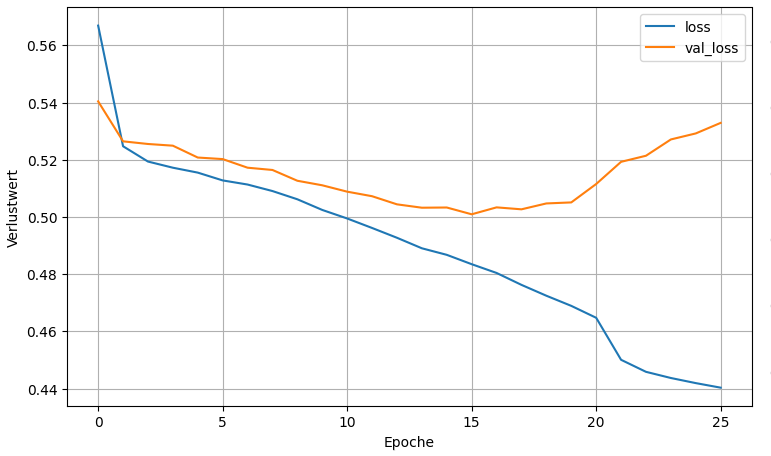
\includegraphics[width=0.8\textwidth,height=8cm,keepaspectratio=true]{content/images/TrainingLoss.png}
    \caption{Entwicklung des Verlustwerts über die Epochen des Trainings}
    \label{fig:TrainingLoss}
\end{figure}

In der Abbildung ist zunächst erkennbar, dass der Verlustwert über die Epochen hinweg optimiert werden kann.
Ab der 15. Epoche beginnt der Verlustwert der Validierung jedoch anzusteigen, während der Verlustwert des Trainings weiter sinkt.
Dieser Effekt spricht für eine Überanpassung.
Dies bedeutet, dass das Modell ab einer bestimmten Epoche beginnt, die Trainingsdaten "`auswendig"' zu lernen.
Dadurch handelt das Modell bei der Validierung jedoch nicht mehr nach den globalen Mustern, wodurch die Vorhersagen anhand der Validierungsdaten schlechter werden.
Der \emph{EarlyStopping}-Callback stellt jedoch den besten Zustand des Modells wieder her, der in diesem Fall bei Epoche 15 bestand.

\subsection{Nachbearbeitung der Vorhersagen}
\label{sec:Nachbearbeitung}
Mit dem trainierten Modell können nun Vorhersagen erzeugt werden.
In \autoref{lst:Prediction} ist dieser Prozess anhand eines zufälligen Beispiels aus den Validierungsdaten gezeigt.

\begin{minipage}{\textwidth}
\begin{code}
\begin{minted}[
    linenos,
    numbersep=10pt,
    gobble=0,
    frame=lines,
    framesep=2mm]{python}
def predict_random_example(model, val_dataset):
    example = val_dataset[np.random.choice(range(len(val_dataset)), size=1)[0]]
    x = np.expand_dims(example[0:-1, ...], axis=0)
    y_true = np.squeeze(example[-1, ...])
    y_pred = np.squeeze(model.predict(x))

    return y_true, y_pred
\end{minted}
\captionof{listing}{Erzeugung einer Vorhersage anhand der Validierungsdaten}
\label{lst:Prediction}
\end{code}
\end{minipage}

Dafür wird in Zeile 1 zunächst eine zufällige Sequenz von 17 Frames aus den Validierungsdaten ausgewählt.
In Zeile 2 und 3 wird die Sequenz in die Eingabe- und Zieldaten unterteilt, die dann jeweils in die richtige Form gebracht werden.
Die eigentliche Vorhersage findet dann in Zeile 5 statt, wo sie durch \emph{model.predict(x)} ausgeführt wird.
Die Arrays \emph{y\_true} und \emph{y\_pred} enthalten nun die wahren und die vorhergesagten Ergebnisse und haben die Form $(50,~50)$.
In \autoref{fig:PredExProb} sind zwei Beispiele für Vorhersagen grafisch dargestellt.

\begin{figure}[h]
    \centering
    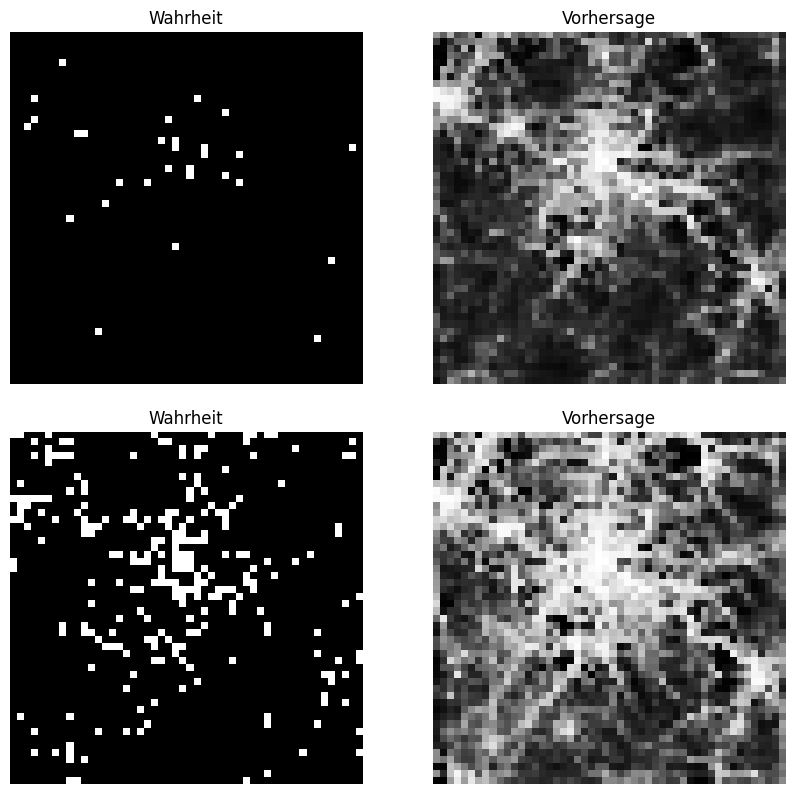
\includegraphics[width=1.0\textwidth,height=12cm,keepaspectratio=true]{content/images/PredExProb.png}
    \caption{Beispiele für Vorhersagen des trainierten Modells (rechts) im Vergleich zur Realität (links)}
    \label{fig:PredExProb}
\end{figure}

Links im Bild sieht man die realen Standorte der mobilen Radarkontrollen.
Rechts hingegen ist die Ausgabe des \acrshortpl{nn} dargestellt.
Je dunkler die Pixel, desto geringer ist der Zahlenwert und umgekehrt.
Zunächst kann man leicht erkennen, dass nicht alle Pixel schwarz sind, sondern dass ein weiter Bereich an Zahlenwerten abgedeckt wird.
Das spricht dafür, dass die gewichtete Verlustfunktion ihren Zweck erfüllt.
Als Nächstes ist erkennbar, dass das Modell scheinbar teilweise das Straßennetz erlernt hat.
In den Vorhersagen sind große Straßen als Linien und große Städte als Cluster deutlich erkennbar.
Dies ist durchaus nachvollziehbar, da die Radarkontrollendichte hier besonders hoch ist.
Dadurch stellt sich jedoch die Frage, ob die Vorhersage des Modells überhaupt maßgeblich von der Eingabe abhängig ist.
Dafür spricht jedenfalls der Unterschied zwischen dem oberen und unteren Beispiel.
Im oberen Beispiel sind in der Realität deutlich weniger Radarkontrollen vorhanden als im unteren Beispiel.
Das könnte beispielsweise dadurch zustande kommen, dass das obere Beispiel von einem Samstag oder Sonntag stammt.
In der bereits diskutierten \autoref{fig:AnzahlNachWochentag} ist schließlich deutlich zu erkennen, dass es am Wochenende deutlich weniger Radarkontrollen gibt als unter der Woche.
Auch die Vorhersage spiegelt diesen Sachverhalt wieder.
Während die Vorhersage im oberen Beispiel viele dunkle Pixel enthält, ist die Vorhersage im unteren Beispiel insgesamt deutlich heller, das Modell geht also insgesamt von einer höheren Wahrscheinlichkeit für mobile Radarkontrollen aus.

Zuletzt ist noch eine offensichtliche Tatsache anzumerken, die aber dennoch wichtig ist, und zwar die Beschaffenheit der Ausgabe des Modells.
Jedes Pixel wird als Zahlenwert zwischen 0 und 1 ausgegeben.
Das liegt an der Aktivierungsfunktion \emph{Sigmoid} des letzten Layers, die die Zahlengerade auf den Bereich zwischen 0 und 1 abbildet.
Der Bereich zwischen 0 und 1 legt nahe, dass die Ausgabe des Modells als Wahrscheinlichkeitskarte angesehen werden kann.
Nun stellt sich die Frage, ob die Ausgabe so belassen oder ob sie noch nachverarbeitet werden sollte.
Hierzu gibt es zwei relevante Aspekte: die praktische Nutzbarkeit und die Performanceevaluierung.
Zur Performanceevaluierung muss beachtet werden, dass die Problemstellung bisher als Binärklassifizierung angesehen wird.
Daher muss die Ausgabe zur Evaluierung wie auch die Eingabe eine Binärklassifizierung sein.
Nur so kann bestimmt werden, wie viele Rasterzellen richtig klassifiziert werden.
Im Bezug auch die praktische Nutzbarkeit ist es durchaus möglich, das Ergebnis als Wahrscheinlichkeit zu belassen.
Jedoch hat diese Vorgehensweise den Nachteil, dass eine Wahrscheinlichkeit unter Umständen schwer einzuschätzen sein kann, besonders in der Hektik des Straßenverkehrs.
Daher bietet es sich an, die ausgegebenen Wahrscheinlichkeiten in mehrere Gefahrenstufen zu unterteilen, die einfach verständlich sind.
Diese Gefahrenstufen könnten beispielsweise \emph{niedrig}, \emph{mittel}, \emph{hoch} und \emph{sehr hoch} heißen.

Unabhängig davon, ob die Wahrscheinlichkeiten als Binärklassifizierung in zwei Stufen aufgeteilt werden soll oder als Gefahrenangabe in mehrere, stellt sich die Frage, wo die Grenzen gesetzt werden sollten.
Eine gute und einfach zu interpretierende Möglichkeit ist die Entscheidung nach Perzentil.
In diesem Fall beziehen sich Perzentile auf die Verteilung der Rasterzellenwerte.
Die 90. Perzentilgrenze liegt beispielsweise so, dass 90\,\% aller Rasterzellen einen Wert unter dieser Grenze haben.
Bei der Wahl der Perzentilgrenze hat im Fall einer Binärklassifizierung eine große Auswirkung auf das Ergebnis.
Dies soll in \autoref{fig:PredExPercentile} verdeutlicht werden.

\begin{figure}[h]
    \centering
    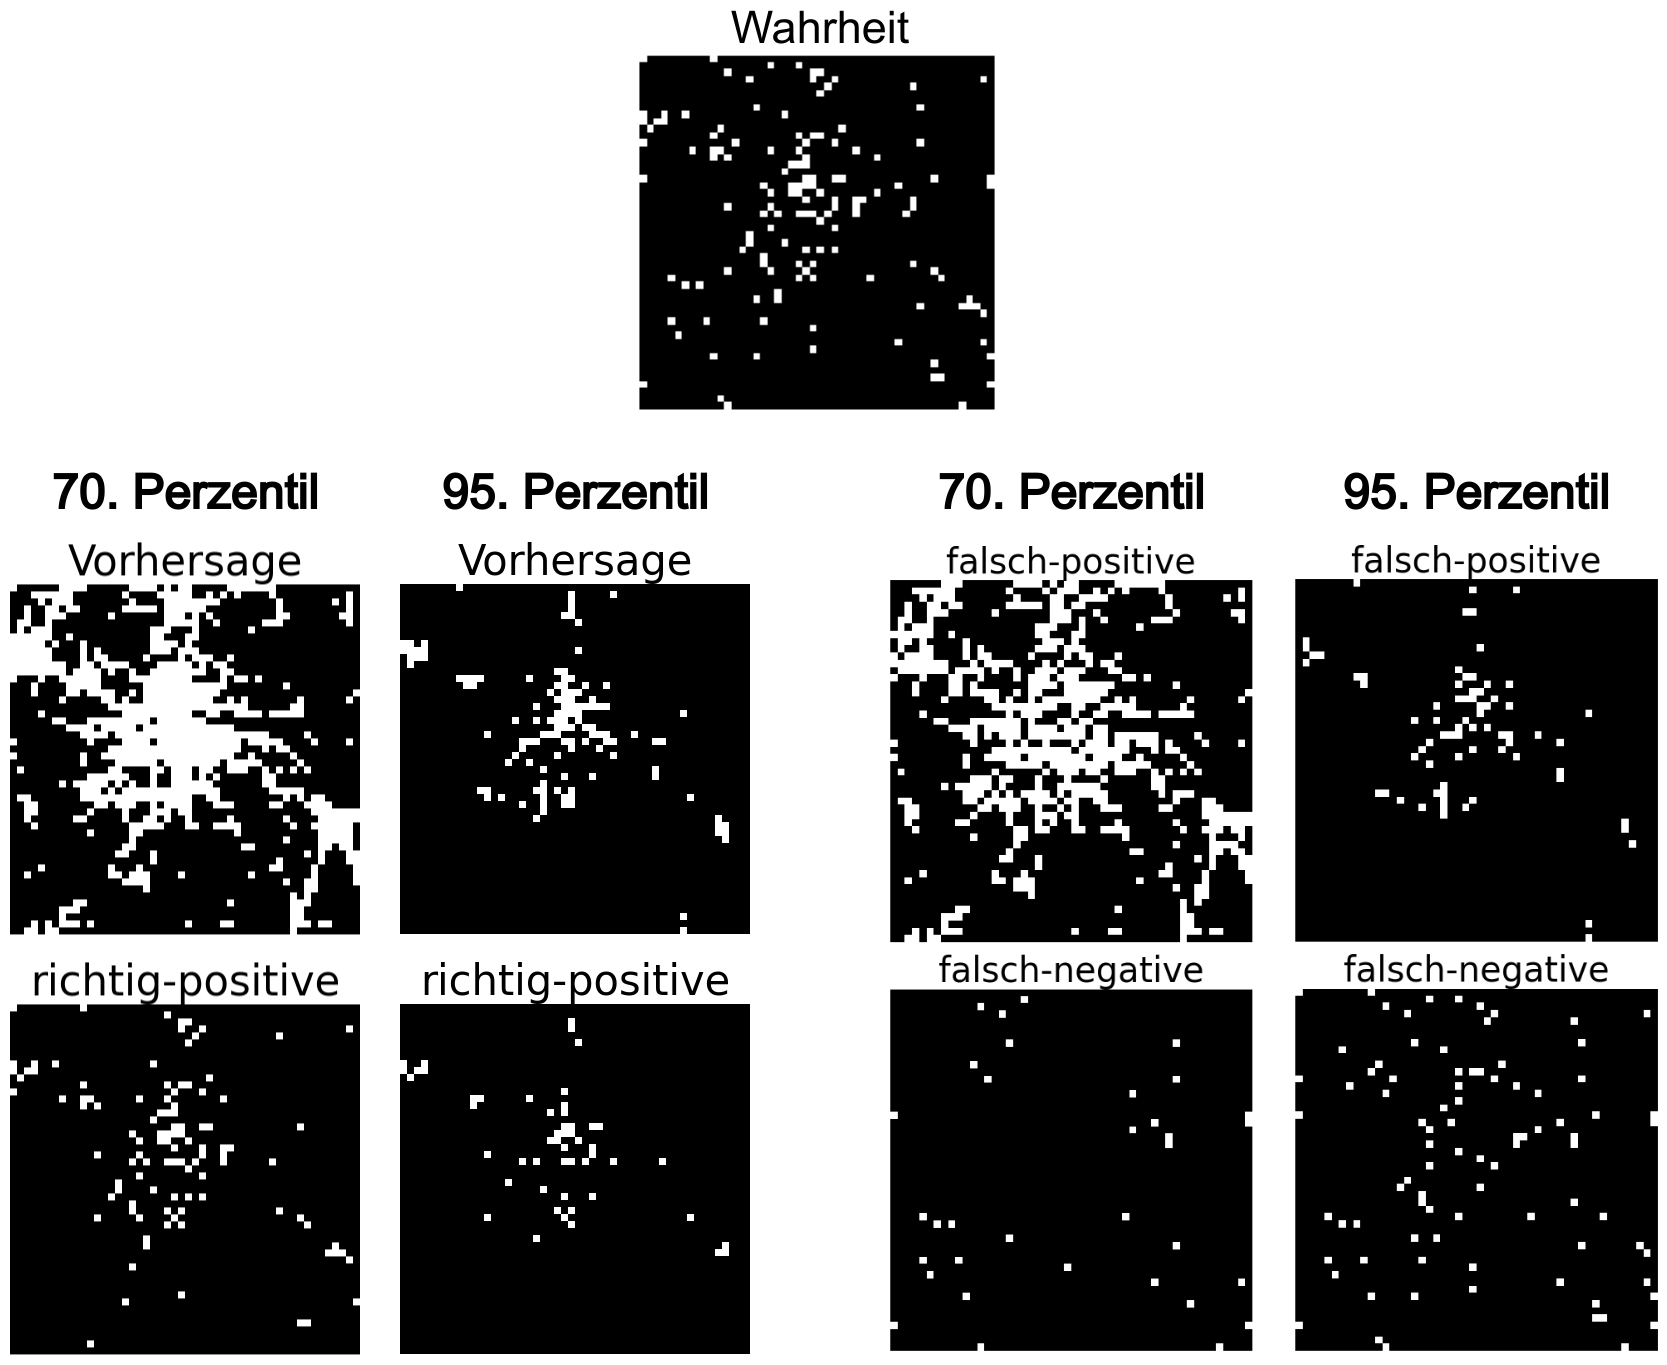
\includegraphics[width=1.0\textwidth,height=12cm,keepaspectratio=true]{content/images/PredExPercentile.png}
    \caption{Auswirkung der Perzentilgrenze auf die Vorhersage im Fall einer Binärklassifizierung}
    \label{fig:PredExPercentile}
\end{figure}

In der Abbildung ist als Beispiel eine Vorhersage bei zwei verschiedenen Perzentilgrenzen zu sehen.
Dabei zeigt das oberste Bild die Grundwahrheit.
Unten ist die Vorhersage je für die 70. und 95. Perzentilgrenze dargestellt.
Außerdem ist die Vorhersage jeweils in die richtig-positiv, falsch-positiv und falsch-negativ vorhergesagten Rasterzellen aufgeschlüsselt.
Im Einklang mit der Definition der Perzentilgrenze ist beim Vergleich der Vorhersagen offensichtlich, dass mit der 70. Perzentilgrenze deutlich mehr Rasterzellen als "`positiv"' eingestuft werden als mit der 95. Perzentilgrenze.
Dies hat zur Folge, dass mit der 70. Perzentilgrenze mehr der tatsächlich positiven Rasterzellen korrekt vorhergesagt werden.
Jedoch resultieren daraus auch deutlich mehr Falsch-Positive.
Stellt man sich dieses Szenario in der Praxis vor, würden Benutzer relativ häufit gewarnt werden, obwohl keine akute Gefahr für Radarkontrollen besteht.
Es lässt sich jedoch argumentieren, dass es in der Praxis wichtiger ist, dass vor so vielen tatsächlich positiven Rasterzellen gewarnt werden sollte wie möglich, auch wenn dadurch Fehlwarnungen häufiger werden.
In \autoref{fig:PredExPercentile} sind bisher nur Beispiele für zwei konkrete Perzentilgrenzen dargestellt.
Für eine genauere Analyse sind jedoch Werte über alle Perzentilgrenzen interessant.
Diese sind als Graphen für dasselbe Beispiel in \autoref{fig:PredExGraphs} dargestellt.

\begin{figure}[h]
    \centering
    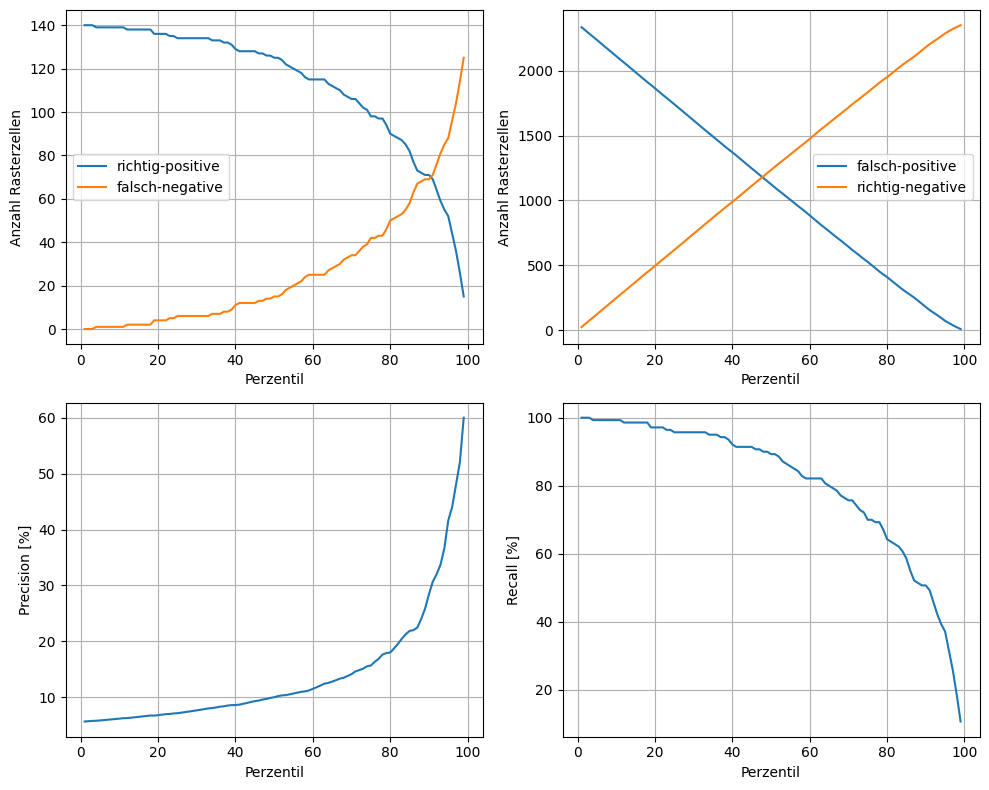
\includegraphics[width=1.0\textwidth,height=12cm,keepaspectratio=true]{content/images/PredExGraphs.png}
    \caption{Verschiedene Metriken einer Beispielvorhersage über Perzentilgrenzen von 1\,\% bis 99\,\%}
    \label{fig:PredExGraphs}
\end{figure}

In den oberen beiden Graphen sind die Kennzahlen, die oben schon für zwei Perzentilgrenzen analysiert wurden, über alle Perzentilgrenzen aufgetragen.
Für die Betrachtung ist wichtig zu wissen, dass es insgesamt 2500 Rasterzellen gibt, von denen in diesem Beispiel in der Realität 140 "`positiv"' sind.
Dies wird auch deutlich, wenn man die linken Enden der Graphen betrachtet.
Bei der nullten Perzentilgrenze werden per Definition alle Zellen als "`positiv"' markiert, weshalb dort auch die Anzahl der Richtig-Positiven maximal ist.
Jedoch ist dort auch die Anzahl der Falsch-Positiven maximal.
Aufgrund der unbalancierten Verteilung der positiven Rasterzellen verhält sich die Richtig-positiven- und Falsch-negativen-Rate über die Perzentilgrenzen hinweg exponentiell, während sich die Falsch-positiven- und Richtig-negativen-Rate annähernd linear verhält.
Zur intuitiveren Bewertung der Perzentilgrenzen sind die absoluten Zahlen wenig aussagekräftig, zumal sie sich bei verschiedenen Beispielen unterschiedlich verhalten.
Daher gibt es verschiedene Metriken, die die absoluten Werte zueinander ins Verhältnis setzen.
Diese werden in \cite{ImbalancedData} beschrieben.
Die einfachste solche Metrik ist die Genauigkeit, die den Anteil der richtig klassifizierten Elemente darstellt, es gilt also
$$
\text{Genauigkeit} = \frac{\text{Korrekt klassifizierte Elemente}}{\text{Gesamtanzahl der Elemente}}.
$$
In \autoref{sec:ModellDefinition} wurde jedoch bereits erörtert, warum die Genauigkeit für unbalancierte Daten nicht aussagekräftig ist.
Deulich hilfreicher sind die Metriken \emph{Precision} und \emph{Recall}.
Precision ist nach \cite{ImbalancedData} der Anteil der positiv vorhergesagten Elemente, die auch in der Realität "`positiv"' sind, es gilt also
$$
\text{Precision} = \frac{\text{Richtig-Positive}}{\text{Richtig-Positive + Falsch-Positive}}.
$$
Recall gibt hingegen an, welcher Anteil der tatsächlich positiven Elemente auch als "`positiv"' erkannt werden.
Hier gilt somit
$$
\text{Recall} = \frac{\text{Richtig-Positive}}{\text{Richtig-Positive + Falsch-Negative}}.
$$
Um diese Metriken genauer zu verstehen, ist es hilfreich zu betrachten, wann sie 100\,\% betragen.
Damit die Precision 100\,\% beträgt, darf es keine Falsch-Positiven geben.
Somit ist die Precision ein Maß dafür, wie präzise \emph{nur} die tatsächlich Positiven erkannt werden.
Wichtig ist hierbei anzumerken, dass die Precision nichts darüber aussagt, wie viele der tatsächlich Positiven erkannt werden.
Die Precision könnte also 100\,\% betragen, obwohl nur wenige Prozent der tatsächlich Positiven erkannt werden.
Wichtig ist nur, dass es keine Falsch-Positiven gibt.
Genau andersherum ist es nun beim Recall.
Der Recall beträgt genau dann 100\,\%, wenn es keine Falsch-Negativen gibt.
Es müssen also alle tatsächlich positiven Elemente erkannt werden.
Dabei ist es jedoch unerheblich, wie viele in der Realität negativen Elemente zusätzlich noch als "`positiv"' erkannt werden.

Insgesamt ist also klar, dass bei der Wahl der Perzentilgrenze zwischen Precision und Recall abgewogen werden muss.
In \autoref{fig:PredExGraphs} sind Precision und Recall in den unteren beiden Graphen für das konkrete Beispiel dargestellt.
Anhand des Precision-Graphs ist zu erkennen, dass selbst mit einer Perzentilgrenze von 99\,\% keine Precision über 60\,\% möglich ist.
Es gibt also immer eine gewisse, nicht zu vernachlässigende Anzahl an Falsch-Positiven.
Außerdem ist erkennbar, dass die Precision-Kurve bei Perzentilgrenzen gegen 99\,\% sehr stark ansteigt.
Die Rasterzellen, die einen Wert in diesem Bereich haben, sind also mit großer Wahrscheinlichkeit tatsächlich "`positiv"'.
Im Bezug auf den Anwendungsfall der Vorhersage von mobilen Radarkontrollen hat die Recall-Kurve eine noch größere Bedeutung, da möglichst viele tatsächlich vorhandene Radarkontrollen in der Vorhersage enthalten sein sollten.
Jedoch bleibt es eine Abwägung zwischen Precision und Recall.
Daher bietet es sich an, beide Metriken in einem Graph in Relation zueinander zu setzen.
Diesen Graph nennt man \acrfull{prc}.
Die \acrshort{prc} der bisher verwendeten Beispielvorhersage ist in \autoref{fig:PredExGraphsPRC} links dargestellt.

\begin{figure}[h]
    \centering
    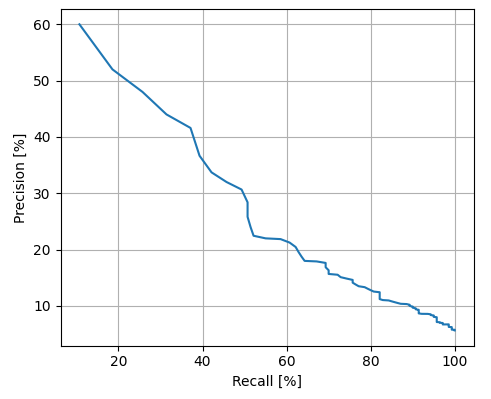
\includegraphics[width=0.7\textwidth,height=8cm,keepaspectratio=true]{content/images/PredExGraphsPRC.png}
    \caption{\acrfull{prc} einer Beispielvorhersage}
    \label{fig:PredExGraphsPRC}
\end{figure}

An diesem Graphen kann abgelesen werden, welche Precision bei welchem Recall erreichbar ist und umgekehrt.
Soll beispielsweise ein Recall von 70\,\% erreicht werden, entspricht dies einer Precision von ca. 15\,\%.
In Worten werden also 70\,\% aller Rasterzellen korrekt vorhergesagt, die tatsächlich eine Radarkontrolle beinhalten, jedoch enthalten nur 15\,\% aller als "`positiv"' vorhergesagten Rasterzellen tatsächlich eine Radarkontrolle.
Wenn die \acrshort{prc} für den gesamten Validierungsdatensatz erstellt wird, eignet sie sich auch dazu, die Performance verschiedener Modelle zu vergleichen.
Falls ein Modell besser performt als ein anderes, liegt die \acrshort{prc} dieses Modells eher weiter oben rechts.
Es ergeben sich also insgesamt größere Precision-Recall-Paare.

Die \acrshort{prc} kann nun gemeinsam mit den einzelnen Graphen von Precision und Recall verwendet werden, um geeignete Perzentilgrenzen für eine Gefahreneinstufung auszuwählen.
Für die Einteilung in die vier Gefahrenstufen \emph{niedrig}, \emph{mittel}, \emph{hoch} und \emph{sehr hoch} müssen drei Perzentilgrenzen ausgewählt werden.
Für die Grenze, ab der die Gefahrenstufe \emph{mittel} gelten soll, scheint das 60. Perzentil ein guter Wert zu sein.
Dies entspricht einem Recall von ca. 82\,\% und einer Precision von ca. 12\,\%.
Der Recall-Wert bedeutet, dass nur 18\,\% der tatsächlichen Radarkontrollen (fälschlicherweise) auf die Gefahrenstufe \emph{niedrig} fallen.
Die Precision ist jedoch nicht sonderlich hoch.
Es befinden sich folglich sehr viele Falsch-Positive in der Gefahrenstufe \emph{mittel}.
Die nächste Gefahrenstufe (für die Gefahrenstufe \emph{hoch}) kann beim 85. Perzentil angelegt werden.
Hier beträgt der Recall ca. 60\,\% und die Precision ca. 23\,\%.
Die Precision hat sich demnach im Vergleich zur Gefahrenstufe \emph{mittel} fast verdoppelt, während der Recall nur um ein Viertel geringer geworden ist.
Bei der Gefahrenstufe \emph{sehr hoch} sollte sich das Modell sehr sicher sein, dass sich in einer solchen Rasterzelle eine Radarkontrolle befindet.
Daher sollte eine Perzentilgrenze nahe 100\,\% gewählt werden, wie beispielsweise die 98. Perzentilgrenze.
Hier beträgt der Recall zwar nur noch ca. 10\,\%, die Precision jedoch ca. 55\,\%.
Statistisch befinden sich demnach in ca. der Hälfte aller Rasterzellen der Gefahrenstufe \emph{sehr hoch} tatsächlich eine Radarkontrolle.

Werden die Gefahrenstufen mit unterschiedlichen Farben markiert, ergibt sich für das bisher verwendete Beispiel die in \autoref{fig:Gefahrenstufen} dargestellte Gefahrenkarte.

\begin{figure}[h]
    \centering
    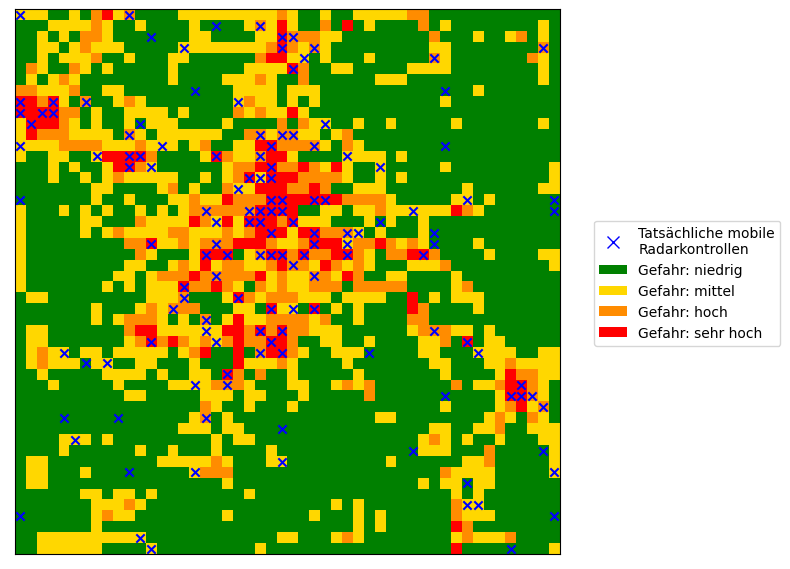
\includegraphics[width=0.7\textwidth,height=8cm,keepaspectratio=true]{content/images/Gefahrenstufen.png}
    \caption{Resultierende nachbearbeitete Vorhersage mit vier Gefahrenstufen im Vergleich zur Grundwahrheit}
    \label{fig:Gefahrenstufen}
\end{figure}

Außerdem sind in der Abbildung die tatsächlichen Radarkontrollen mit einem Kreuz markiert.
Wird einem Autofahrer bei jedem Rasterzellenwechsel die neue Gefahrenstufe mitgeteilt, kann dieser sie leichter einschätzen und sich entsprechend verhalten.

\subsection{Evaluierung des Modells}
\label{sec:Evaluierung}
In diesem Abschnitt werden zunächst Metriken festgelegt, mit denen die Performance des Modells unter verschiedenen Bedingungen verglichen werden können.
Anschließend wird die Performance des Modells anhand der Validierungsdaten evaluiert, indem untersucht wird, inwiefern die Vorhersagen des Modells von den konkreten Eingabeframes abhängen.

Zunächst gilt es Metriken zu definieren, anhand derer das Modell unter verschiedenen Bedingungen verglichen werden kann.
Da Precision und Recall von der Perzentilgrenze abhängig sind, eignen sie sich nicht direkt.
Was sich hingegen eignet, ist die Precision-Recall-Kurve, da sie Precision und Recall über alle Perzentilgrenzen hinweg darstellt.
Zwei \acrshortpl{prc} können verglichen werden, indem ermittelt wird, welche Kurve über der anderen liegt.
Jedoch erfolgt die Interpretation grafisch, obwohl der Vergleich von einzelnen Zahlenwerten oft einfacher ist.
Außerdem könnte bei verschiedenen Recall-Werten eine unterschiedliche Kurve die höhere Precision haben.
Eine Möglichkeit, eine komplette \acrshort{prc} in einem Zahlenwert zusammenzufassen, besteht darin, die Fläche unter der Kurve zu berechnen.
Dieser Wert wird \acrfull{auprc} genannt.
Mit der \acrshort{auprc} kann die Performance eines Modells mit einer Zahl beschrieben werden und zwei Modelle können somit einfach verglichen werden.

Anhand der \acrshort{prc} und der \acrshort{auprc} soll nun zunächst das in den vorherigen Abschnitten implementierte Modell evaluiert werden.
Dabei soll auch eine der Kernfragen der vorliegenden Arbeit beantwortet werden.
Diese Kernfrage ist, ob sich die Standorte von mobilen Radarkontrollen anhand von historischen Daten und insbesondere derer der letzten 16 Tage vorhersagen lassen.
Besonders interessant ist hierbei, inwieweit die Vorhersagen konkret von den 16 Eingabeframes abhängt.
Wenn die Ausgabe praktisch unabhängig von den Eingabeframes wäre, würde eine rein statistische Auswertung des Datensatzes für die Vorhersagen genügen, wie z.\,B. die Identifizierung von Hotspots.
Um das Ausmaß der Abhängigkeit zu ermitteln, bietet es sich an, die Zielframes zufällig zu vertauschen.
Somit kann überprüft werden, ob die Vorhersagen des Modells mit einem zufällig ausgewählten Zielframe genau so gut übereinstimmen wie mit dem Zielframe des tatsächlichen nächsten Tages.
Wenn dem so ist, sind die Vorhersagen weitestgehend unabhängig von den konkreten Eingabeframes.
Erzielt das Modell jedoch bessere Ergebnisse mit den wahren Zielframes, ist eine Abhängigkeit bestätigt.
Bevor die Überprüfung durchgeführt werden kann, sollte jedoch die Wahl des Validierungsdatensatzes angepasst werden.
In \autoref{sec:DatensatzLaden} wurde bisher definiert, dass sich die Sequenzen des Datensatzes beliebig überschneiden können, um eine größere Menge an Trainingsdaten zu erhalten.
Die erzeugten Sequenzen wurden dann zufällig dem Trainings- und Validierungsdatensatz zugewiesen.
Dies hat zur Folge, dass sich die Sequenzen des Trainings- und Validierungsdatensatzes u.\,U. nur um zwei Frames unterscheiden - das Erste und das Letzte.
Dies hat auch zur Folge, dass die Zielframes des Validierungsdatensatzes im Trainingsdatensatz vorhanden sein können.
Somit hätte das Modell die Zielframes der Validierung schon gesehen, was die Evaluierung der Abhängigkeit verfälschen würde.
Um sicherzustellen, dass dies nicht der Fall ist, werden die nach dem Anfangsdatum sortierten Sequenzen zunächst in Gruppen von je 34 Sequenzen unterteilt.
Da dieser Wert der doppelten Sequenzlänge inklusive der Zielframes entspricht, überschneiden sich die Gruppen nicht.
Als Nächstes werden die Sequenzgruppen gemischt und zufällig in Trainings- und Validierungsdaten unterteilt.
Zuletzt werden die Trainings- und Validierungsdaten nochmals in sich gemischt.
Mit diesen korrigierten Datensätzen muss das Modell nun erneut trainiert werden und die Evaluierung mit gemischten Zielframes kann durchgeführt werden.
Die daraus resultierenden \acrshortpl{prc} sind in \autoref{fig:PRCValGetrennt} zu sehen.
Außerdem sind die \acrshort{auprc}-Werte der Kurven in der Legende aufgeführt.

\begin{figure}[h]
    \centering
    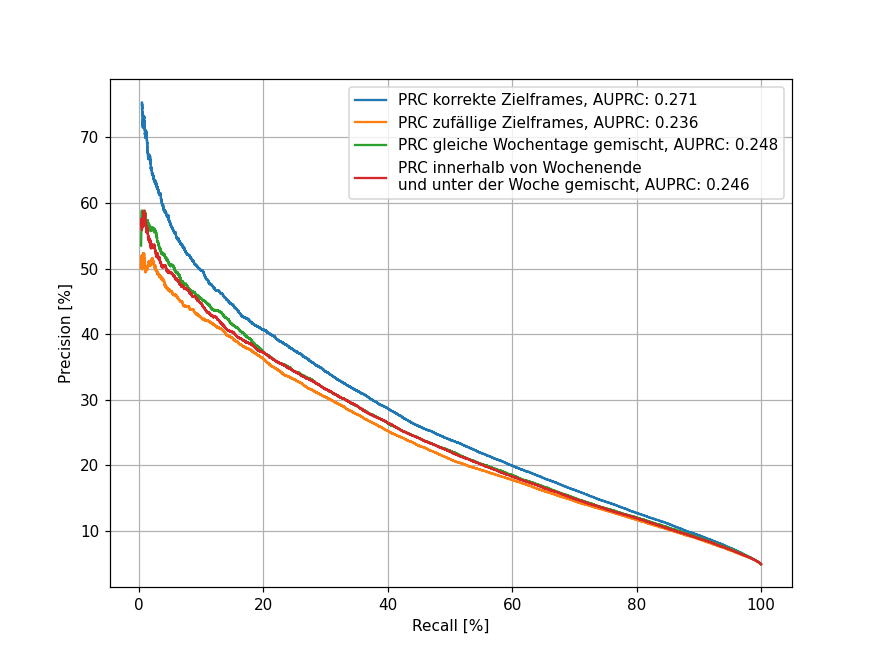
\includegraphics[width=1.0\textwidth,height=12cm,keepaspectratio=true]{content/images/PRCValGetrennt.png}
    \caption{\acrshortpl{prc} und \acrshort{auprc}-Werte mit wahren und gemischten Zielframes}
    \label{fig:PRCValGetrennt}
\end{figure}

Hierbei ist anzumerken, dass die \acrshortpl{prc} den Durchschnitt des gesamten Validierungsdatensatzes darstellen und nicht wie in \autoref{fig:PredExGraphsPRC} nur eine einzelne Vorhersage.
Dadurch verlaufen die Kurven weicher und gleichmäßiger.
Es ist deutlich zu erkennen, dass die mit den zufälligen Zielframes erzeugte \acrshort{prc} (orange) am niedrigsten liegt und auch den geringsten \acrshort{auprc}-Wert von 0,236 aufweist.
Die \acrshort{prc} mit den korrekten Zielframes liegt hingegen höher.
Dadurch erfährt auch der \acrshort{auprc}-Wert einen Zuwachs von ca. 15\,\% und liegt somit bei 0,271.

Im vorherigen Abschnitt wurde bereits aufgezeigt, dass das Modell den Unterschied zwischen Wochenende und unter der Woche gut erlernen kann.
Dieser Unterschied ist jedoch sehr einfach zu erkennen, da es am Wochenende durchschnittlich nur halb so viele Radarkontrollen gibt wie unter der Woche.
Daher ist es für die Evaluierung interessant, diesen Effekt bei der Analyse auszuschließen.
Dies kann realisiert werden, indem nur die Samstage und Sonntage untereinander gemischt werden, wie auch die Tage Montag bis Freitag.
Es kann auch noch einen Schritt weiter gegangen werden, indem nur gleiche Wochentage gemischt werden.
Hierdurch werden jedoch u.\,U. wochentagabhängige Muster unterdrückt, die eine durchaus valide Leistung des Modells darstellen.
Andererseits kann mit diesem Vorgehen untersucht werden, ob überhaupt wochentagabhängige Muster in den Daten existieren.
Daher sind in \autoref{fig:PRCValGetrennt} beide Ansätze dargestellt.
Es ist erkennbar, dass die Kurven wie erwartet etwas über der Kurve der komplett zufälligen Zielframes liegt.
Daraus kann abgeleitet werden, dass das Modell tatsächlich den Unterschied zwischen Wochenende und unter der Woche gelernt hat.
Jedoch liegen die Kurven immer noch deutlich unter der Kurve der korrekten Zielframes.
Daraus folgt, dass es im Datensatz noch weitere Muster gibt, die über den Unterschied zwischen Wochenende und unter der Woche hinaus gehen und dass die gewählte Modellarchitektur fähig ist, diese zu erlernen.
Bei den Kurven ist besonders der linke Rand interessant, da dies der Bereich ist, in dem sich das Modell mit den Vorhersagen sehr sicher ist.
Daher ist dieser Bereich in \autoref{fig:PRCValGetrenntZoom} vergrößert dargestellt.

\begin{figure}[h]
    \centering
    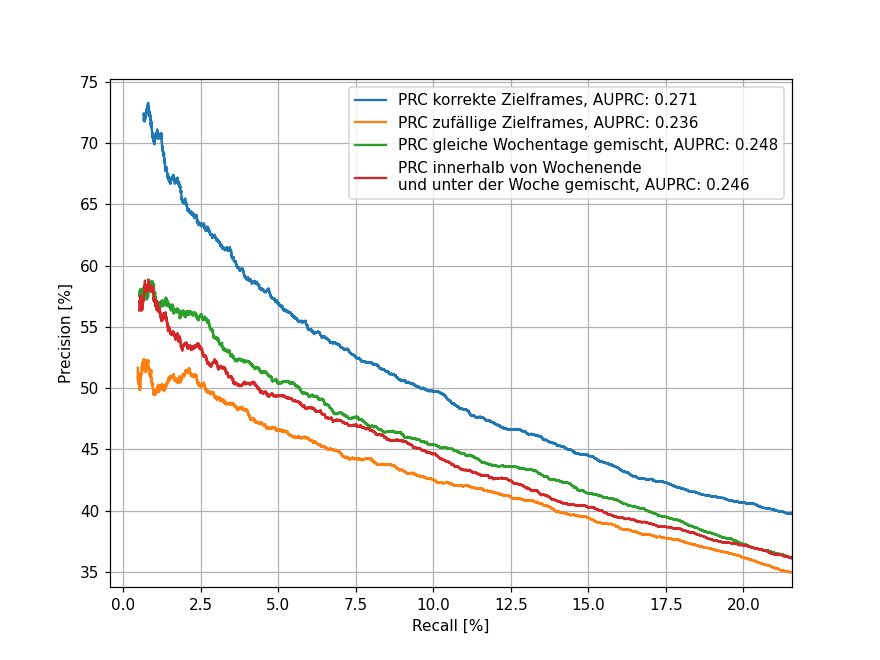
\includegraphics[width=1.0\textwidth,height=12cm,keepaspectratio=true]{content/images/PRCValGetrenntZoom.png}
    \caption{\acrshortpl{prc} im Detail bei geringen Recall- und hohen Precision-Werten}
    \label{fig:PRCValGetrenntZoom}
\end{figure}

Der dargestellte Bereich entspricht einer Perzentilgrenze von etwa 96\,\% am rechten Rand bis 99,5\,\% am linken Rand.
Hier bestätigt sich die Vermutung, dass es wochentagabhängige Muster in den Daten gibt, da die grüne Kurve, für die nur gleiche Wochentage gemischt wurden, etwas über der roten Kurve liegt.
Die Signifikanz dieses Unterschieds ist jedoch diskutabel.
Zusammenfassend bestätigt die durchgeführte Evaluierung, dass es verschiedene Muster in den Daten gibt und dass das Modell dazu in der Lage ist, diese Muster zu erlernen.

